We present an additional experiment to evaluate our proposed mini-batch \textsc{SAGD}.

In this section, we consider a Natural Language Inference task on the Stanford Natural Language Inference (SNLI) dataset~\citep{bowman2015large}. 
The SNLI corpus is a collection of $570 \, 000$ human-written English sentence pairs manually labeled for balanced classification.
The goal is to predict if an hypothesis sentence is an \emph{entailment}, \emph{contradiction} or \emph{neutral} with respect to a given text.
This task of natural language inference (NLI) is also known as recognizing textual entailment. 

\textbf{Dataset and Evaluation Metrics:} 
For SNLI, all training samples are used to train the model and we report the training perplexity and the test perplexity across~epochs. 
Cross-entropy is used as the loss function throughout experiments. 
The mini-batch size is set to 20 for this dataset. 
We repeat each experiment 5 times and report the mean and standard deviation of the results.



\textbf{Model and Hyperparameters:} 
We use a bi-directional LSTM architecture, as the concatenation of a forward LSTM and a backward LSTM as described in \citep{conneau2017supervised}.
We use 300 dimensions as fixed word embeddings and set the learning rate following the method described in the main paper.


\begin{figure}[H] 
 \mbox{
%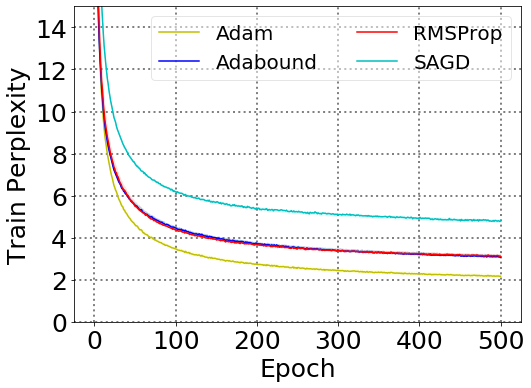
\includegraphics[width = 0.48 \textwidth ]{figure/bilstmtrain.png}
%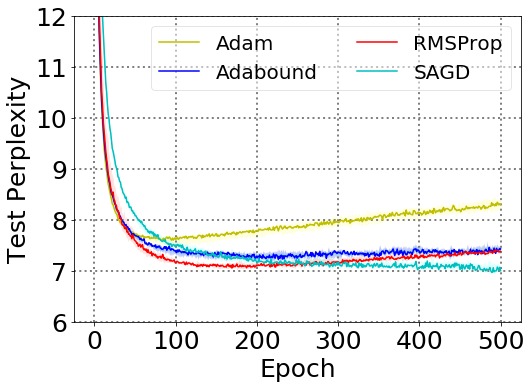
\includegraphics[width = 0.48 \textwidth ]{figure/bilstmtest.png}
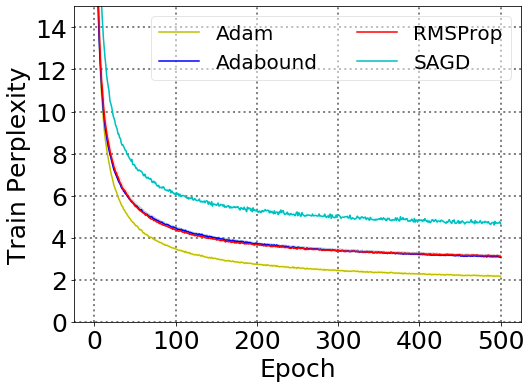
\includegraphics[width = 0.48 \textwidth ]{figure/bilstmtrainwithlap.png}
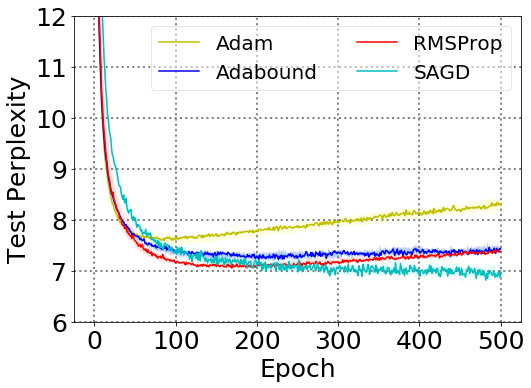
\includegraphics[width = 0.48 \textwidth ]{figure/bilstmtestwithlap.png}
 }
 \vspace{-0.1in}
 \caption[]{Train and test perplexity of biLSTM on SNLI. 
 \textsc{SAGD} performs the best in terms of the test perplexity among all the methods while showing a worse loss perplexity. SAGD empirically avoids over-fitting.
} 
 \label{fig:snli}\vspace{-0.05in}
\end{figure}

In Figure~\ref{fig:snli}, we compare mini-batch SAGD to the following baselines: Adam~\citep{kiba15},  RMSprop~\citep{tige12}, and Adabound~\citep{luxi2019}. 
As in the NLP task on Penn Treebank, we observe that whilst SAGD displays a worse loss perplexity than its competition, it succeeds in keeping a low testing perplexity through the epochs.
This phenomena has been observed in all of our experiments (either classification of images or inference of text) and highlights the advantage of our proposed method to present \emph{reused} samples to the model as if they were fresh ones. 
Thus, over-fitting is less likely to happen and testing loss will remain low.
As an example of over-fitting, we observe in In Figure~\ref{fig:snli} that Adam achieves the best training perplexity, yet displays an increasing testing perplexity after only a few epochs, which leads to bad final test accuracy.